% The contents of this file is 
% Copyright (c) 2009-  Charles R. Severance, All Righs Reserved

\chapter{Visualización de datos}

Hasta el momento, hemos estudiado en primer lugar el lenguaje de Python y luego
hemos descubierto cómo usar Python, la red y las bases de datos
para manipular datos.

En este capítulo, echaremos un vistazo a tres
aplicaciones completas que reúnen todas esas cosas
para gestionar y visualizar datos. Puedes usar estas aplicaciones
como código de ejemplo que te puede servir de punto de partida para la
resolución de problemas del mundo real.

Cada una de las aplicaciones es un archivo ZIP que puedes descargar,
extraer en tu equipo y ejecutar.

\section{Construcción de un mapa de Google a partir de datos geocodificados}
\index{Google!mapa}
\index{Visualización!mapa}

En este proyecto usaremos la API de geocodificación de Google
para limpiar varias ubicaciones geográficas de nombres de universidades
introducidas por los usuarios, y luego colocaremos los datos en
un mapa de Google. 

\beforefig
\centerline{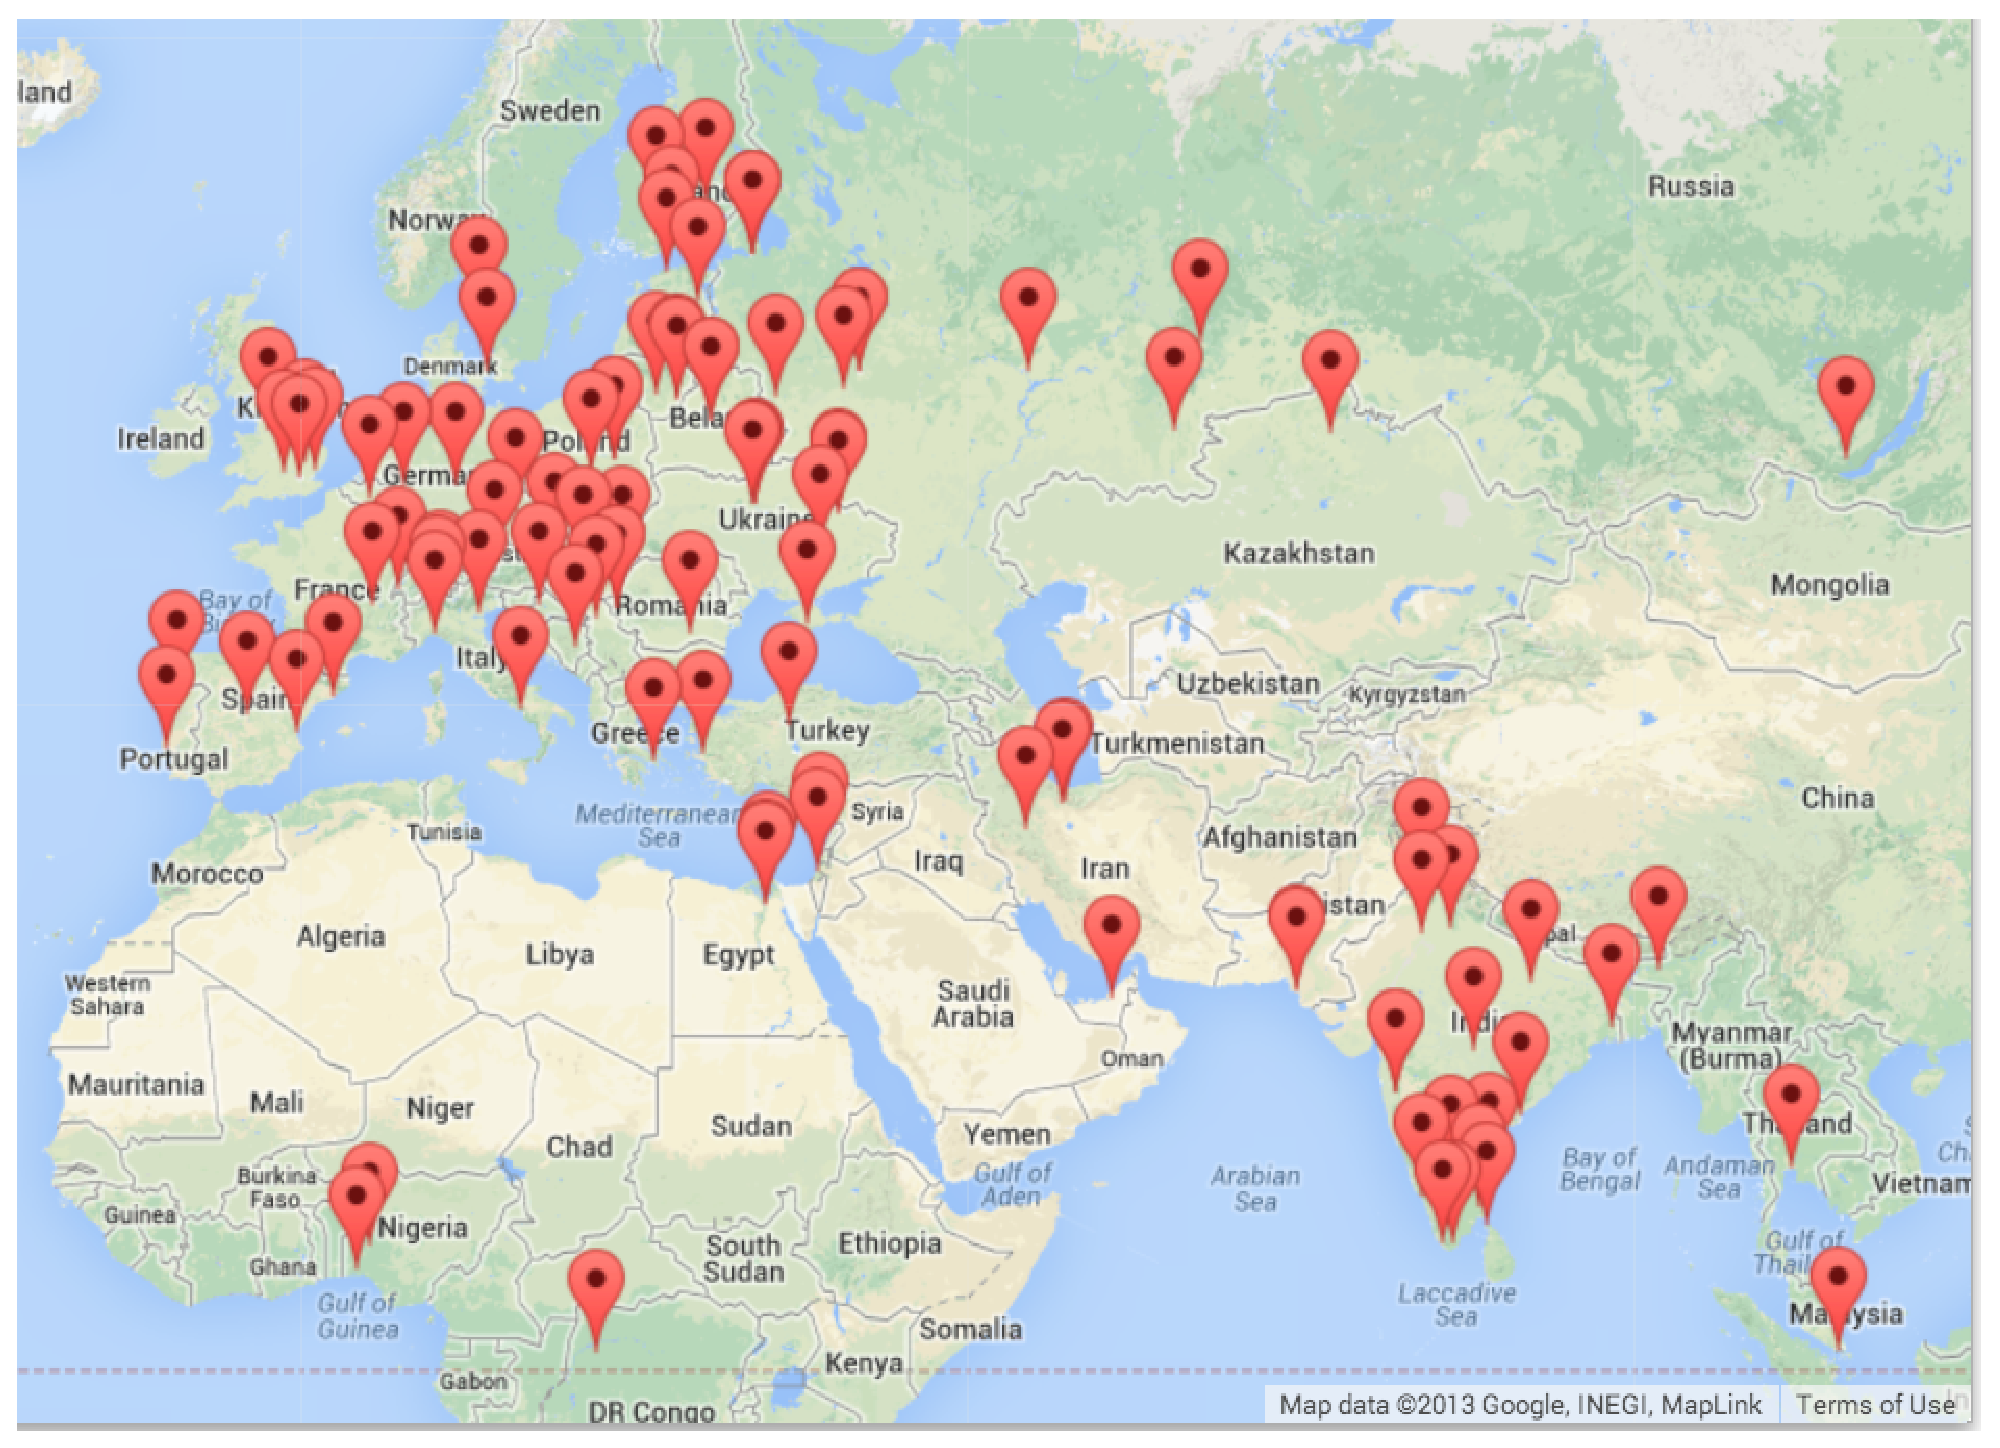
\includegraphics[height=2.25in]{figs2/google-map.eps}}
\afterfig

Para comenzar, descarga la aplicación desde:

\url{www.py4inf.com/code/geodata.zip}

El primer problema a resolver es que la API libre de geocodificación
de Google tiene como límite de uso un cierto número de peticiones diarias. Si tienes
un montón de datos, necesitarás detener y reanudar el proceso de
búsqueda varias veces. De modo que dividiremos el problema en
dos fases.

\index{caché}
En la primera fase, tomaremos como entrada los datos ``de reconocimiento'' del archivo
{\bf where.data} y los leeremos línea a línea, recuperando la
información de geocodificación desde Google y almacenándola
en una base de datos {\bf geodata.sqlite}.
Antes de usar la API de geocodificación para cada ubicación introducida por los usuarios,
verificaremos si ya tenemos los datos para esa entrada
concreta. La base de datos funcionará así como una ``caché'' local
de datos de geocodificación, para asegurarnos de que nunca solicitamos
a Google los mismos datos dos veces.

Puedes reiniciar el proceso en cualquier momento eliminando el archivo
{\bf geodata.sqlite}.

Ejecuta el programa {\bf geoload.py}. Este programa leerá las líneas
de entrada desde {\bf where.data} y para cada línea verificará primero si ya
está en la base de datos. Si no disponemos de datos para esa ubicación,
llamará a la API de geocodificación para recuperarlos y los almacenará
en la base de datos.

Aquí tenemos un ejemplo de ejecución cuando ya disponemos de alguna información almacenada en la
base de datos:

\beforeverb
\begin{verbatim}
Found in database  Northeastern University
Found in database  University of Hong Kong, ...
Found in database  Technion
Found in database  Viswakarma Institute, Pune, India
Found in database  UMD
Found in database  Tufts University

Resolving Monash University
Retrieving http://maps.googleapis.com/maps/api/
    geocode/json?sensor=false&address=Monash+University
Retrieved 2063 characters {    "results" : [  
{u'status': u'OK', u'results': ... }

Resolving Kokshetau Institute of Economics and Management
Retrieving http://maps.googleapis.com/maps/api/
    geocode/json?sensor=false&address=Kokshetau+Inst ...
Retrieved 1749 characters {    "results" : [  
{u'status': u'OK', u'results': ... }
...
\end{verbatim}
\afterverb
%
Las primeras cinco ubicaciones ya están en la base de datos y por eso
las omitimos. El programa explora hasta que encuentra ubicaciones
nuevas y entonces comienza a recuperarlas.

El programa {\bf geoload.py} puede ser detenido en cualquier momento, y dispone de un
contador que puedes usar para limitar el número de llamadas a la API de geolocalización
en cada ejecución. Dado que el fichero {\bf where.data} sólo tiene unos pocos cientos
de elementos, no deberías llegar al límite diario de usos, pero si
tienes más datos pueden ser necesarias varias ejecuciones del programa durante varios días
para conseguir tener todos los datos de entrada geolocalizados en nuestra base de datos.

Una vez que tienes parte de los datos cargados en {\bf geodata.sqlite}, se pueden
visualizar usando el programa {\bf geodump.py}. Este
programa lee la base de datos y escribe el arhivo {\bf where.js}
con la ubicación, latitud y longitud en forma de
código ejecutable JavaScript.

Una ejecución del programa {\bf geodump.py} sería la siguiente: 

\beforeverb
\begin{verbatim}
Northeastern University, ... Boston, MA 02115, USA 42.3396998 -71.08975
Bradley University, 1501 ... Peoria, IL 61625, USA 40.6963857 -89.6160811
...
Technion, Viazman 87, Kesalsaba, 32000, Israel 32.7775 35.0216667
Monash University Clayton ... VIC 3800, Australia -37.9152113 145.134682
Kokshetau, Kazakhstan 53.2833333 69.3833333
...
12 records written to where.js
Open where.html to view the data in a browser
\end{verbatim}
\afterverb
%
El archivo {\bf where.html} consiste en HTML y JavaScript para mostrar
un mapa de Google. Lee los datos más actuales de {\bf where.js} para obtener
los datos que se visualizarán. He aquí el formato del fichero {\bf where.js}:

\beforeverb
\begin{verbatim}
myData = [
[42.3396998,-71.08975, 'Northeastern Uni ... Boston, MA 02115'],
[40.6963857,-89.6160811, 'Bradley University, ... Peoria, IL 61625, USA'],
[32.7775,35.0216667, 'Technion, Viazman 87, Kesalsaba, 32000, Israel'],
   ...
];
\end{verbatim}
\afterverb
%
Se trata de una variable JavaScript que contiene una lista de listas.
La sintaxis de las listas de constantes en JavaScript es muy similar a
las de Python, de modo que ésta debería resultarte familiar.

Simplemente abre {\bf where.html} en un navegador para ver las ubicaciones.
Puedes mantener el ratón sobre cada marca del mapa para ver la
ubicación que la API de geocodificación ha devuelto para la entrada que el usuario introdujo.
Si no puedes ver ningún dato cuando abras el fichero {\bf where.html}, deberás
verificar que tengas activado JavaScript o usar la consola de desarrollador de tu navegador.

\section{Visualización de redes e interconexiones}
\index{Google!clasificación de páginas}
\index{Visualización!redes}
\index{Visualización!clasificación de páginas}

En la siguiente aplicación, realizaremos algunas de las funciones de un motor
de búsqueda. Primero rastrearemos una pequeña parte de la web y ejecutaremos
una versión simplificada del algoritmo de clasificación que usa la página de Google
para determinar qué páginas son las más visitadas. Luego visualizaremos
la clasificación de las páginas y visitas de nuestro pequeño rincón de la web.
Usaremos la librería de visualización de JavaScript D3
\url{http://d3js.org/} para generar la imagen de salida.

Puedes descargar y extraer esta aplicación desde:

\url{www.py4inf.com/code/pagerank.zip}

\beforefig
\centerline{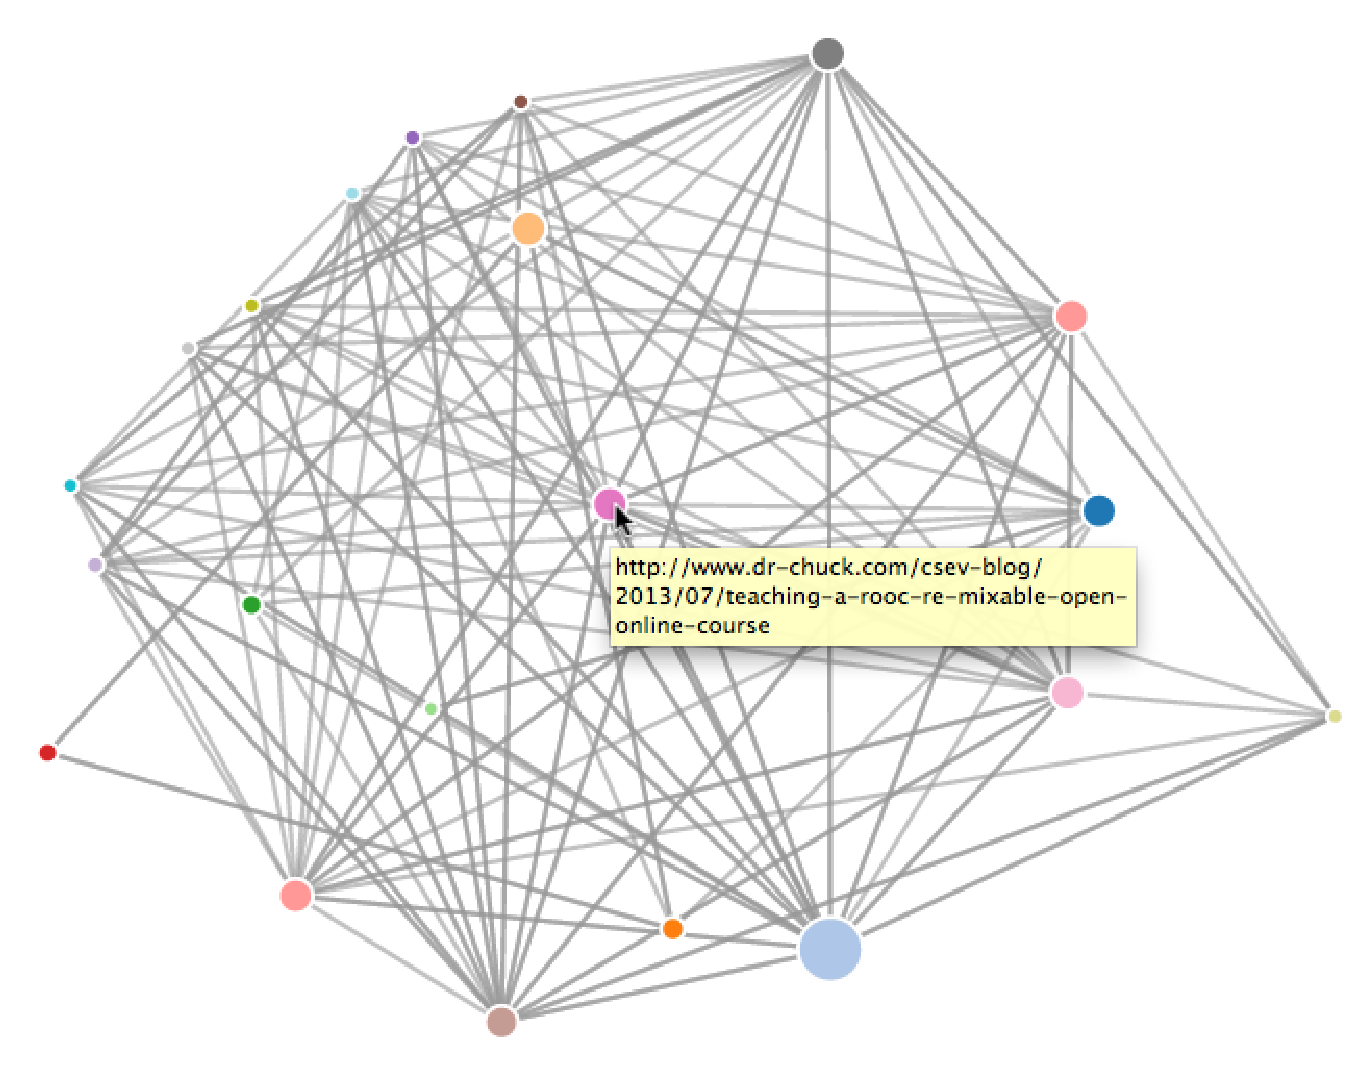
\includegraphics[height=2.25in]{figs2/pagerank.eps}}
\afterfig

El primer programa ({\bf spider.py}) rastrea un sitio web
y envía una serie de páginas a la
base de datos ({\bf spider.sqlite}), guardando los enlaces entre páginas.
Puedes reiniciar el proceso en cualquier momento eliminando el
fichero {\bf spider.sqlite} y ejecutando de nuevo {\bf spider.py}.

\beforeverb
\begin{verbatim}
Enter web url or enter: http://www.dr-chuck.com/
['http://www.dr-chuck.com']
How many pages:2
1 http://www.dr-chuck.com/ 12
2 http://www.dr-chuck.com/csev-blog/ 57
How many pages:
\end{verbatim}
\afterverb
%
En esta ejecución de ejemplo, le pedimos que rastree un sitio web y que recupere dos
páginas. Si reinicias el programa y le pides que rastree más
páginas, no volverá a revisar aquellas que ya estén en la base de datos.
En cada reinicio elegirá una página al azar no rastreada aún y comenzará allí.
De modo que cada ejecución sucesiva de {\bf spider.py} irá añadiendo páginas nuevas.

\beforeverb
\begin{verbatim}
Enter web url or enter: http://www.dr-chuck.com/
['http://www.dr-chuck.com']
How many pages:3
3 http://www.dr-chuck.com/csev-blog 57
4 http://www.dr-chuck.com/dr-chuck/resume/speaking.htm 1
5 http://www.dr-chuck.com/dr-chuck/resume/index.htm 13
How many pages:
\end{verbatim}
\afterverb
%
Se pueden tener múltiples puntos de partida en la misma base de datos---dentro
del programa, éstos son llamados ``webs''. La araña
elije entre todos los enlaces no visitados de las páginas existentes uno al azar
como siguiente página a rastrear.

Si quieres ver el contenido del fichero {\bf spider.sqlite}, puedes
ejecutar {\bf spdump.py}, que mostrará algo como esto:

\beforeverb
\begin{verbatim}
(5, None, 1.0, 3, u'http://www.dr-chuck.com/csev-blog')
(3, None, 1.0, 4, u'http://www.dr-chuck.com/dr-chuck/resume/speaking.htm')
(1, None, 1.0, 2, u'http://www.dr-chuck.com/csev-blog/')
(1, None, 1.0, 5, u'http://www.dr-chuck.com/dr-chuck/resume/index.htm')
4 rows.
\end{verbatim}
\afterverb
%
Se muestra el número de enlaces hacia la página, la clasificación antigua de la página, la
clasificación nueva, el id de la página, y la url de la página. El programa {\bf spdump.py}
sólo muestra aquellas páginas que tienen al menos un enlace hacia ella.

Una vez que tienes unas cuantas páginas en la base de datos, puedes ejecutar el clasificador sobre ellas, usando el programa {\bf sprank.py}. Simplemente debes indicarle cuántas
iteraciones del clasificador de páginas debe realizar.

\beforeverb
\begin{verbatim}
How many iterations:2
1 0.546848992536
2 0.226714939664
[(1, 0.559), (2, 0.659), (3, 0.985), (4, 2.135), (5, 0.659)]
\end{verbatim}
\afterverb
%
Puedes volcar en pantalla el contenido de la base de datos de nuevo para ver que la clasificación de
páginas ha sido actualizada:

\beforeverb
\begin{verbatim}
(5, 1.0, 0.985, 3, u'http://www.dr-chuck.com/csev-blog')
(3, 1.0, 2.135, 4, u'http://www.dr-chuck.com/dr-chuck/resume/speaking.htm')
(1, 1.0, 0.659, 2, u'http://www.dr-chuck.com/csev-blog/')
(1, 1.0, 0.659, 5, u'http://www.dr-chuck.com/dr-chuck/resume/index.htm')
4 rows.
\end{verbatim}
\afterverb
%
Puedes ejecutar {\bf sprank.py} tantas veces como quieras, y simplemente irá refinando
la clasificación de páginas cada vez más. Puedes incluso ejecutar {\bf sprank.py} varias veces,
luego ir a la araña {\bf spider.py} a recuperar unas cuantas páginas más y después ejecutar de nuevo
{\bf sprank.py} para actualizar los valores de clasificación. Un motor de búsqueda normalmente
ejecuta ambos programas (el rastreador y el clasificador) de forma constante.

Si quieres reiniciar los cálculos de clasificación de páginas sin tener que rastrear de nuevo
las páginas web, puedes usar {\bf spreset.py} y después reiniciar {\bf sprank.py}.

\beforeverb
\begin{verbatim}
How many iterations:50
1 0.546848992536
2 0.226714939664
3 0.0659516187242
4 0.0244199333
5 0.0102096489546
6 0.00610244329379
...
42 0.000109076928206
43 9.91987599002e-05
44 9.02151706798e-05
45 8.20451504471e-05
46 7.46150183837e-05
47 6.7857770908e-05
48 6.17124694224e-05
49 5.61236959327e-05
50 5.10410499467e-05
[(512, 0.0296), (1, 12.79), (2, 28.93), (3, 6.808), (4, 13.46)]
\end{verbatim}
\afterverb
%
En cada iteración del algoritmo de clasificación de páginas se muestra el cambio
medio en la clasificación de cada página. La red al principio está bastante
desequilibrada, de modo que los valores de esos cambios medios de clasificación
para cada página variarán a lo loco entre iteraciones. Pero después de unas cuantas
iteraciones, la clasificación de páginas converge. Deberías
ejecutar {\bf prank.py} durante el tiempo suficiente para que los valores de clasificación
converjan.

Si quieres visualizar las páginas mejor clasificadas hasta ese momento,
ejecuta {\bf spjson.py} para leer desde base de datos y escribir el ranking de
las páginas más enlazadas en formato JSON, que puede ser visualizado en
un navegador web.

\beforeverb
\begin{verbatim}
Creating JSON output on spider.json...
How many nodes? 30
Open force.html in a browser to view the visualization
\end{verbatim}
\afterverb
%
Puedes ver esos datos abriendo el fichero {\bf force.html} en tu navegador.
Mostrará un diseño automático de los nodos y enlaces. Puedes pinchar y
arrastrar cualquier nodo y también hacer doble click sobre él para ver la URL
que representa.

Si vuelves a ejecutar las otras utilidades, ejecuta de nuevo {\bf spjson.py} y
pulsa ``recargar'' en el navegador para obtener los datos actualizados desde {\bf spider.json}.

\section{Visualización de datos de correo}

Si has llegado hasta este punto del libro, ya debes de estar bastante familiarizado con
nuestros ficheros de datos {\bf mbox-short.txt} y {\bf mbox.txt}. Ahora es el momento
de llevar nuestro análisis de datos de correo electrónico al siguiente nivel.

En el mundo real, a veces se tienen que descargar datos de correo desde los servidores.
Eso podría llevar bastante tiempo y los datos podrían tener inconsistencias,
estar llenos de errores, y necesitar un montón de limpieza y ajustes. En esta sección,
trabajaremos con la aplicación más compleja que hemos visto hasta ahora, que
descarga casi un gigabyte de datos y los visualiza.

\beforefig
\centerline{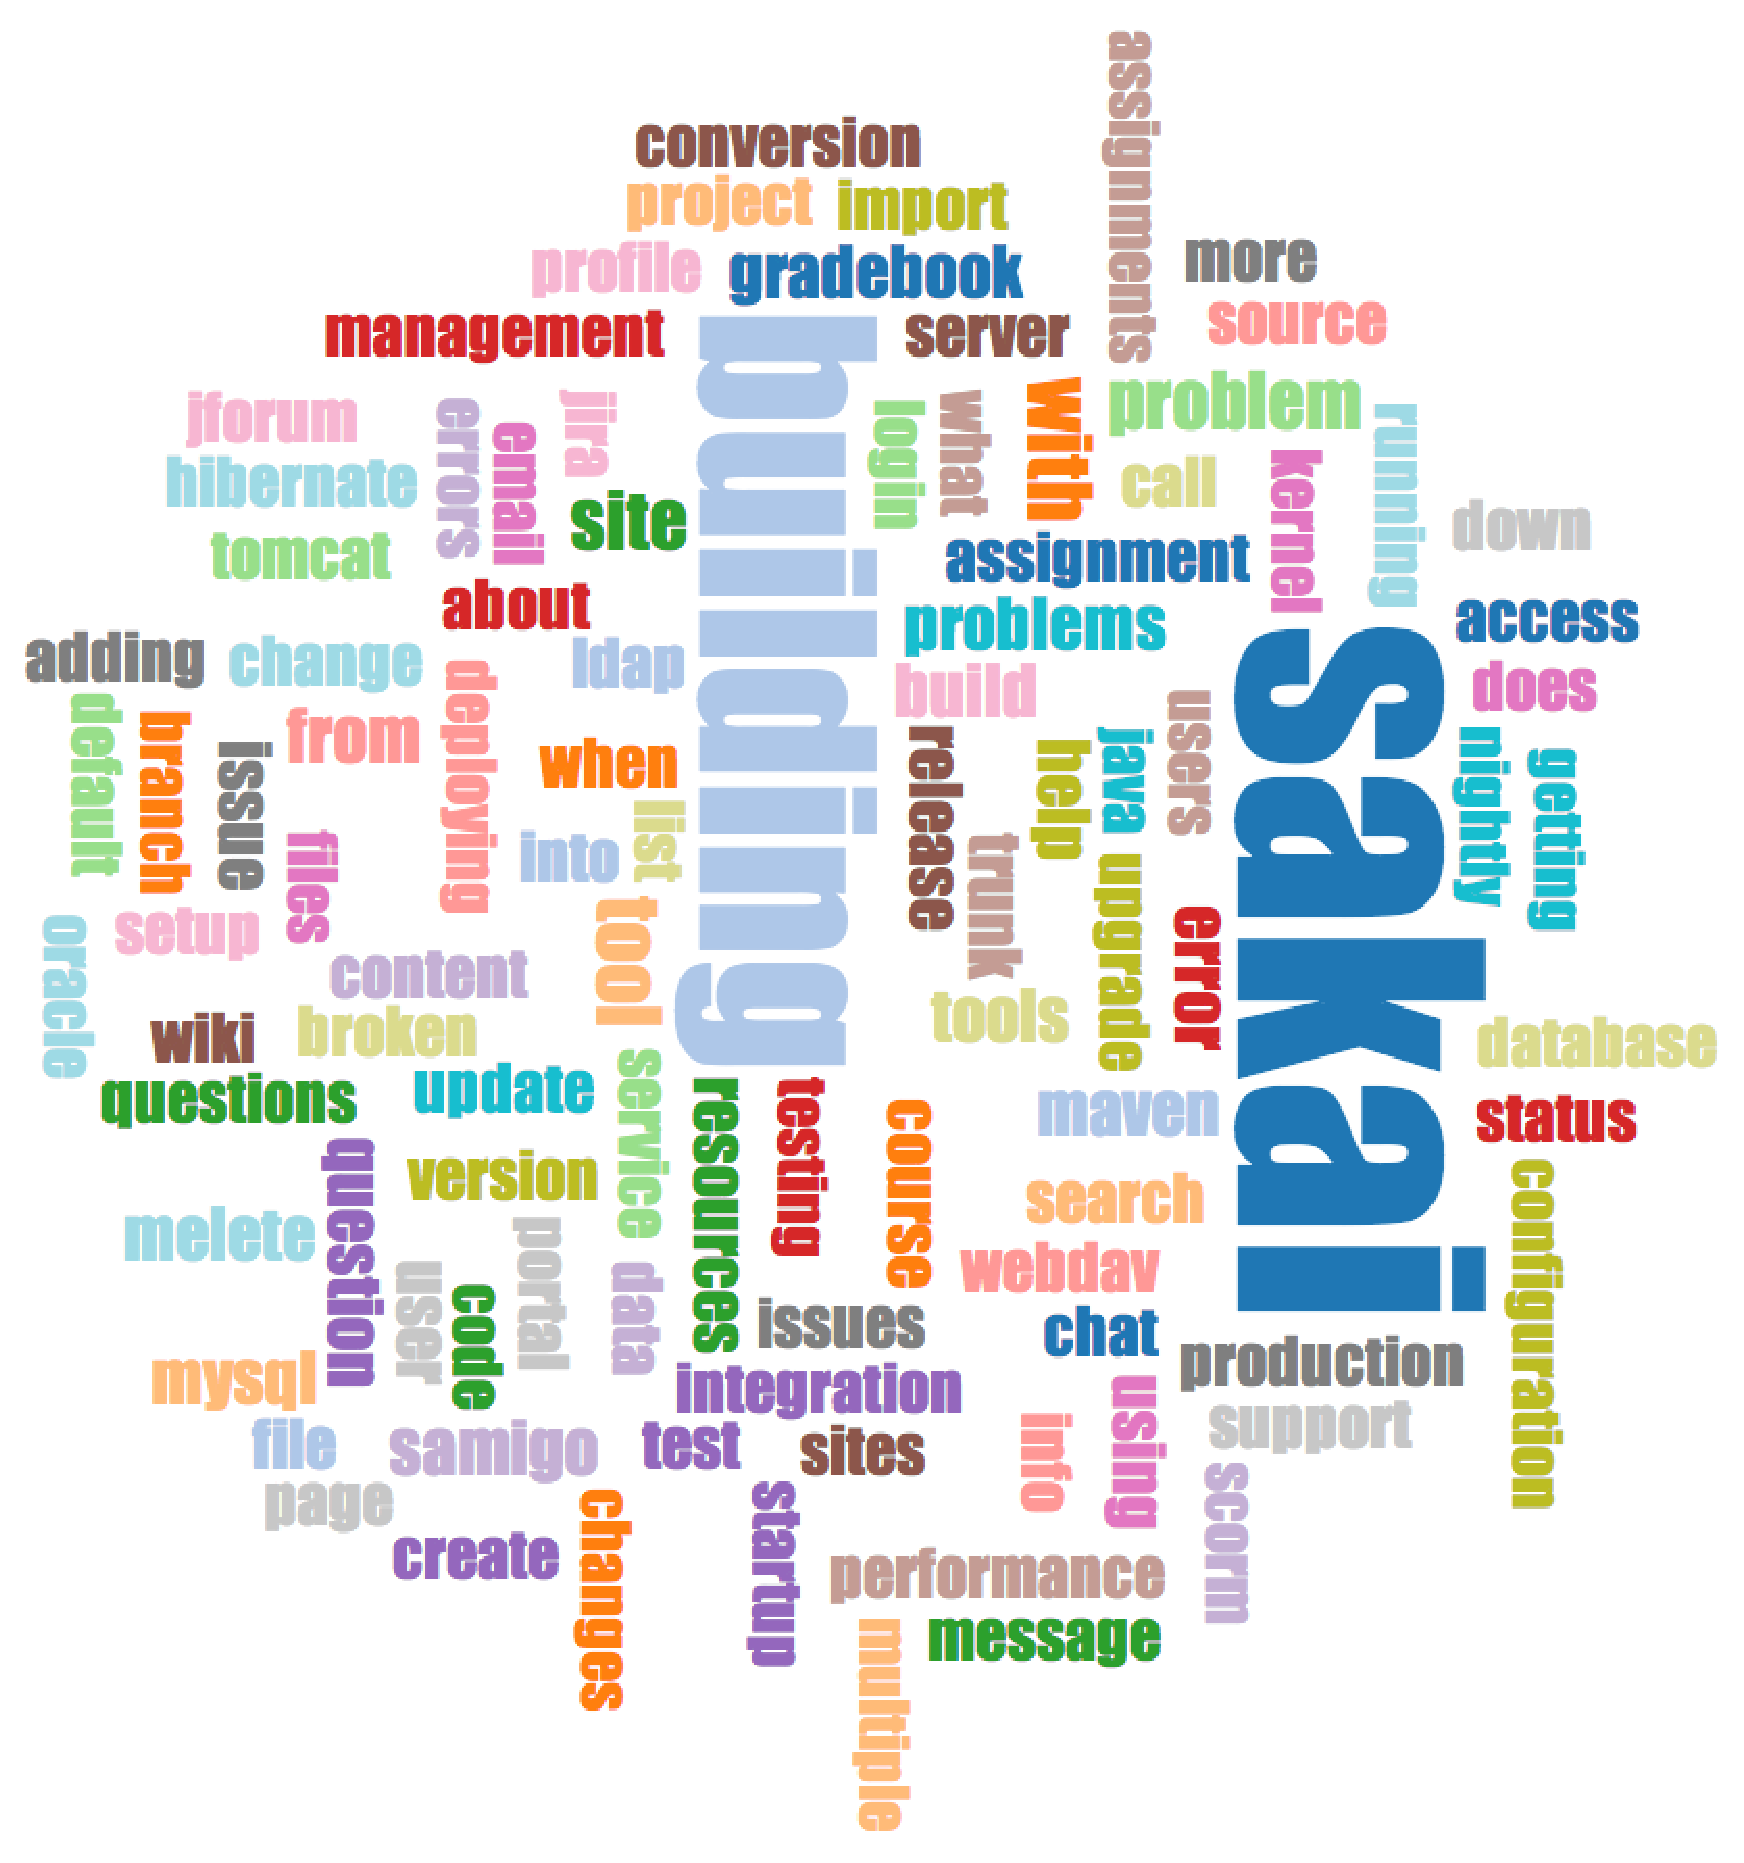
\includegraphics[height=2.50in]{figs2/wordcloud.eps}}
\afterfig

Puedes descargar la aplicación desde:

\url{www.py4inf.com/code/gmane.zip}

Utilizaremos los datos de un servicio de archivo de listas de correo electrónico libre,
llamado \url{www.gmane.org}. Este servicio es muy popular en proyectos de código abierto,
debido a que proporciona un buen almacenaje con capacidad de búsqueda de su
actividad de correo. También tienen una política muy liberal respecto al acceso a
los datos a través de su API. No tienen límites de acceso, pero te piden que no
sobrecargues su servicio y descargues sólo aquellos datos que necesites. Puedes leer
los términos y condiciones de gmane en su página:

\url{http://gmane.org/export.php}

{\em Es muy importante que hagas uso de los datos de gname.org con
responsabilidad, añadiendo retrasos en tus accesos a sus servicios y extendiendo
la realización de los procesos de larga duración a periodos de tiempo lo suficientemente largos.
No abuses de este servicio libre y lo estropees para los demás.}

Cuando se usa este software para rastrear los datos de correo de Sakai, se genera casi
un Gigabyte de datos y se necesita una cantidad considerable de ejecuciones durante varios días.
El archivo {\bf README.txt} del ZIP anterior contiene instrucciones sobre cómo
descargar una copia pre-rastreada del fichero {\bf content.sqlite} con
la mayor parte del contenido de los correos de Sakai, de modo que no tengas que rastrear
durante cinco días sólo para hacer funcionar los programas. Aunque descargues el contenido
pre-rastreado, deberías ejecutar el proceso de rastreo para recuperar los
mensajes más recientes.

El primer paso es rastrear el repositorio gmane. La URL base
se puede modificar en {\bf gmane.py}, y por defecto apunta a la lista
de desarrolladores de Sakai. Puedes rastrear otro repositorio cambiando la
url base. Asegúrate de borrar el fichero {\bf content.sqlite} si realizas
el cambio de url.

El fichero {\bf gmane.py} opera como una araña caché responsable, que
funciona despacio y recupera un mensaje de correo por segundo para
evitar ser bloqueado por gmane. Almacena todos sus datos
en una base de datos y puede ser interrumpido y reanudado tantas veces como
sean necesarias. Puede llevar muchas horas descargar todos los datos.
De modo que tendrás que reanudarlo varias veces.

He aquí una ejecución de {\bf gmane.py} recuperando los últimos cinco mensajes de
la lista de desarrolladores de Sakai:

\beforeverb
\begin{verbatim}
How many messages:10
http://download.gmane.org/gmane.comp.cms.sakai.devel/51410/51411 9460
    nealcaidin@sakaifoundation.org 2013-04-05 re: [building ...
http://download.gmane.org/gmane.comp.cms.sakai.devel/51411/51412 3379
    samuelgutierrezjimenez@gmail.com 2013-04-06 re: [building ...
http://download.gmane.org/gmane.comp.cms.sakai.devel/51412/51413 9903
    da1@vt.edu 2013-04-05 [building sakai] melete 2.9 oracle ...
http://download.gmane.org/gmane.comp.cms.sakai.devel/51413/51414 349265
    m.shedid@elraed-it.com 2013-04-07 [building sakai] ...
http://download.gmane.org/gmane.comp.cms.sakai.devel/51414/51415 3481
    samuelgutierrezjimenez@gmail.com 2013-04-07 re: ...
http://download.gmane.org/gmane.comp.cms.sakai.devel/51415/51416 0

Does not start with From 
\end{verbatim}
\afterverb
%
El programa revisa {\bf content.sqlite} desde el principio hasta que encuentra un número de mensaje que
aún no ha sido rastreado y comienza a partir de ahí. Continúa rastreando
hasta que ha recuperado el número deseado de mensajes o hasta que llega a una página
que no contiene un mensaje adecuadamente formateado.

A veces \url{gmane.org} no encuentra un mensaje. Tal vez los administradores lo borraron,
o quizás simplemente se perdió. Si tu araña se detiene, y parece que se atasca en
un mensaje que no puede localizar, entra en el SQLite Manager, añade una fila con el id perdido y los
demás campos en blanco y reanuda {\bf gmane.py}. Así se desbloqueará el
proceso de rastreo y podrá continuar. Esos mensajes vacíos serán ignorados en la siguiente
fase del proceso.

Algo bueno es que una vez que has rastreado todos los mensajes y los tienes en
{\bf content.sqlite}, puedes ejecutar {\bf gmane.py} otra vez para obtener los mensajes
nuevos según van siendo enviados a la lista.

Los datos en {\bf content.sqlite} están guardados en bruto, con un modelado de datos
ineficiente y sin comprimir.
Esto se ha hecho así intencionadamente, para permitirte echar un vistazo en {\bf content.sqlite}
usando el SQLite Manager y depurar problemas con el proceso de rastreo.
Sería mala idea ejecutar cualquier consulta sobre esta base de datos, ya que
puede resultar bastante lenta.

El segundo proceso consiste en ejecutar el programa {\bf gmodel.py}. Este programa lee los datos
en bruto de {\bf content.sqlite} y produce una versión limpia y bien modelada de los datos,
que envía al fichero {\bf index.sqlite}. Este fichero es mucho más pequeño (puede ser 10 veces
menor) que {\bf content.sqlite}, porque también comprime la cabecera y el texto del cuerpo.

Cada vez que {\bf gmodel.py} se ejecuta, borra y reconstruye {\bf index.sqlite}, permitiéndote
ajustar sus parámetros y editar las tablas de asignación de {\bf content.sqlite} para ajustar el
proceso de limpieza de datos. Esto es un ejemplo de ejecución de {\bf gmodel.py}. El programa imprime
una línea en pantalla cada vez que son procesados 250 mensajes de correo para que puedas ver su
evolución, ya que puede quedarse funcionando durante un buen rato mientras procesa alrededor de
un Gigabyte de datos de correo.

\beforeverb
\begin{verbatim}
Loaded allsenders 1588 and mapping 28 dns mapping 1
1 2005-12-08T23:34:30-06:00 ggolden22@mac.com
251 2005-12-22T10:03:20-08:00 tpamsler@ucdavis.edu
501 2006-01-12T11:17:34-05:00 lance@indiana.edu
751 2006-01-24T11:13:28-08:00 vrajgopalan@ucmerced.edu
...
\end{verbatim}
\afterverb
%
El programa {\bf gmodel.py} realiza varias labores de limpieza de datos.

Los nombres de dominio son truncados a dos niveles para .com, .org, .edu y .net.
Otros nombres de dominio son truncados a tres niveles. De modo que {\tt si.umich.edu} se transforma en
{\tt umich.edu}, y {\tt caret.cam.ac.uk} queda como {\tt cam.ac.uk}. Las direcciones de correo electrónico también
son transformadas a minúsculas, y algunas de las direcciones de {\tt @gmane.org}, como las siguientes

\beforeverb
\begin{verbatim}
   arwhyte-63aXycvo3TyHXe+LvDLADg@public.gmane.org
\end{verbatim}
\afterverb
%
son convertidas en direcciones reales, cuando esa dirección de correo real existe
en otra parte del cuerpo del mensaje.

En la base de datos {\bf content.sqlite} existen dos tablas que te permiten
asignar tanto nombres de dominios como direcciones de correo individuales que van cambiando
a lo largo del tiempo de existencia de la lista de correo. Por ejemplo, Steve Githens ha usado las
direcciones de correo siguientes, según iba cambiando de trabajo a lo largo del tiempo de existencia
de la lista de desarrolladores de Sakai:

\beforeverb
\begin{verbatim}
s-githens@northwestern.edu
sgithens@cam.ac.uk
swgithen@mtu.edu
\end{verbatim}
\afterverb
%
Podemos añadir dos entradas en la tabla de asignación ({\tt Mapping}) de {\bf content.sqlite}, de modo
que {\bf gmodel.py} enlazará las tres direcciones en una:

\beforeverb
\begin{verbatim}
s-githens@northwestern.edu ->  swgithen@mtu.edu
sgithens@cam.ac.uk -> swgithen@mtu.edu
\end{verbatim}
\afterverb
%
Puedes crear entradas similares en la tabla DNSMapping si hay múltiples nombres
DNS que quieres asignar a una única DNS. En los datos de Sakai se ha realizado la siguiente asignación:

\beforeverb
\begin{verbatim}
iupui.edu -> indiana.edu
\end{verbatim}
\afterverb
%
de modo que todas las cuentas de los distintos campus de las Universidades de Indiana son
seguidas juntas.

Puedes volver a ejecutar {\bf gmodel.py} una y otra vez mientras vas mirando los datos, y añadir
asignaciones para hacer que los datos queden más y más limpios. Cuando lo hayas hecho, tendrás una bonita
versión indexada del correo en {\bf index.sqlite}. Éste es el fichero que usaremos para
analizar los datos. Con ese fichero, el análisis de datos se realizará muy rápidamente.

El primer y más sencillo análisis de datos consistirá en determinar ``¿quién ha enviado más correos?'',
y ``¿qué organización ha enviado más correos?''. Esto se realizará usando {\bf gbasic.py}:

\beforeverb
\begin{verbatim}
How many to dump? 5
Loaded messages= 51330 subjects= 25033 senders= 1584

Top 5 Email list participants
steve.swinsburg@gmail.com 2657
azeckoski@unicon.net 1742
ieb@tfd.co.uk 1591
csev@umich.edu 1304
david.horwitz@uct.ac.za 1184

Top 5 Email list organizations
gmail.com 7339
umich.edu 6243
uct.ac.za 2451
indiana.edu 2258
unicon.net 2055
\end{verbatim}
\afterverb
%
Fijate cómo {\bf gbasic.py} funciona mucho más rápido que {\bf gmane.py},
e incluso que {\bf gmodel.py}. Todos trabajan con los mismos datos, pero
{\bf gbasic.py} está usando los datos comprimidos y normalizados de
{\bf index.sqlite}. Si tienes un montón de datos que gestionar, un proceso
multipaso como el que se realiza en esta aplicación puede ser más largo de desarrollar,
pero te ahorrará un montón de tiempo cuando realmente comiences a explorar
y visualizar los datos.

Puedes generar una vista sencilla con la frecuencia de cada palabra en las
líneas de título, usando el archivo {\bf gword.py}:

\beforeverb
\begin{verbatim}
Range of counts: 33229 129
Output written to gword.js
\end{verbatim}
\afterverb
%
Esto genera el archivo {\bf gword.js}, que puedes visualizar utilizando
{\bf gword.htm} para producir una nube de palabras similar a la del comienzo
de esta sección. 

{\bf gline.py} genera también una segunda vista. En este caso cuenta la participación
en forma de correos de las organizaciones a lo largo del tiempo.

\beforeverb
\begin{verbatim}
Loaded messages= 51330 subjects= 25033 senders= 1584
Top 10 Oranizations
['gmail.com', 'umich.edu', 'uct.ac.za', 'indiana.edu', 
'unicon.net', 'tfd.co.uk', 'berkeley.edu', 'longsight.com', 
'stanford.edu', 'ox.ac.uk']
Output written to gline.js
\end{verbatim}
\afterverb
%
Su salida es guardada en {\bf gline.js}, que se puede visualizar usando {\bf gline.htm}.

\beforefig
\centerline{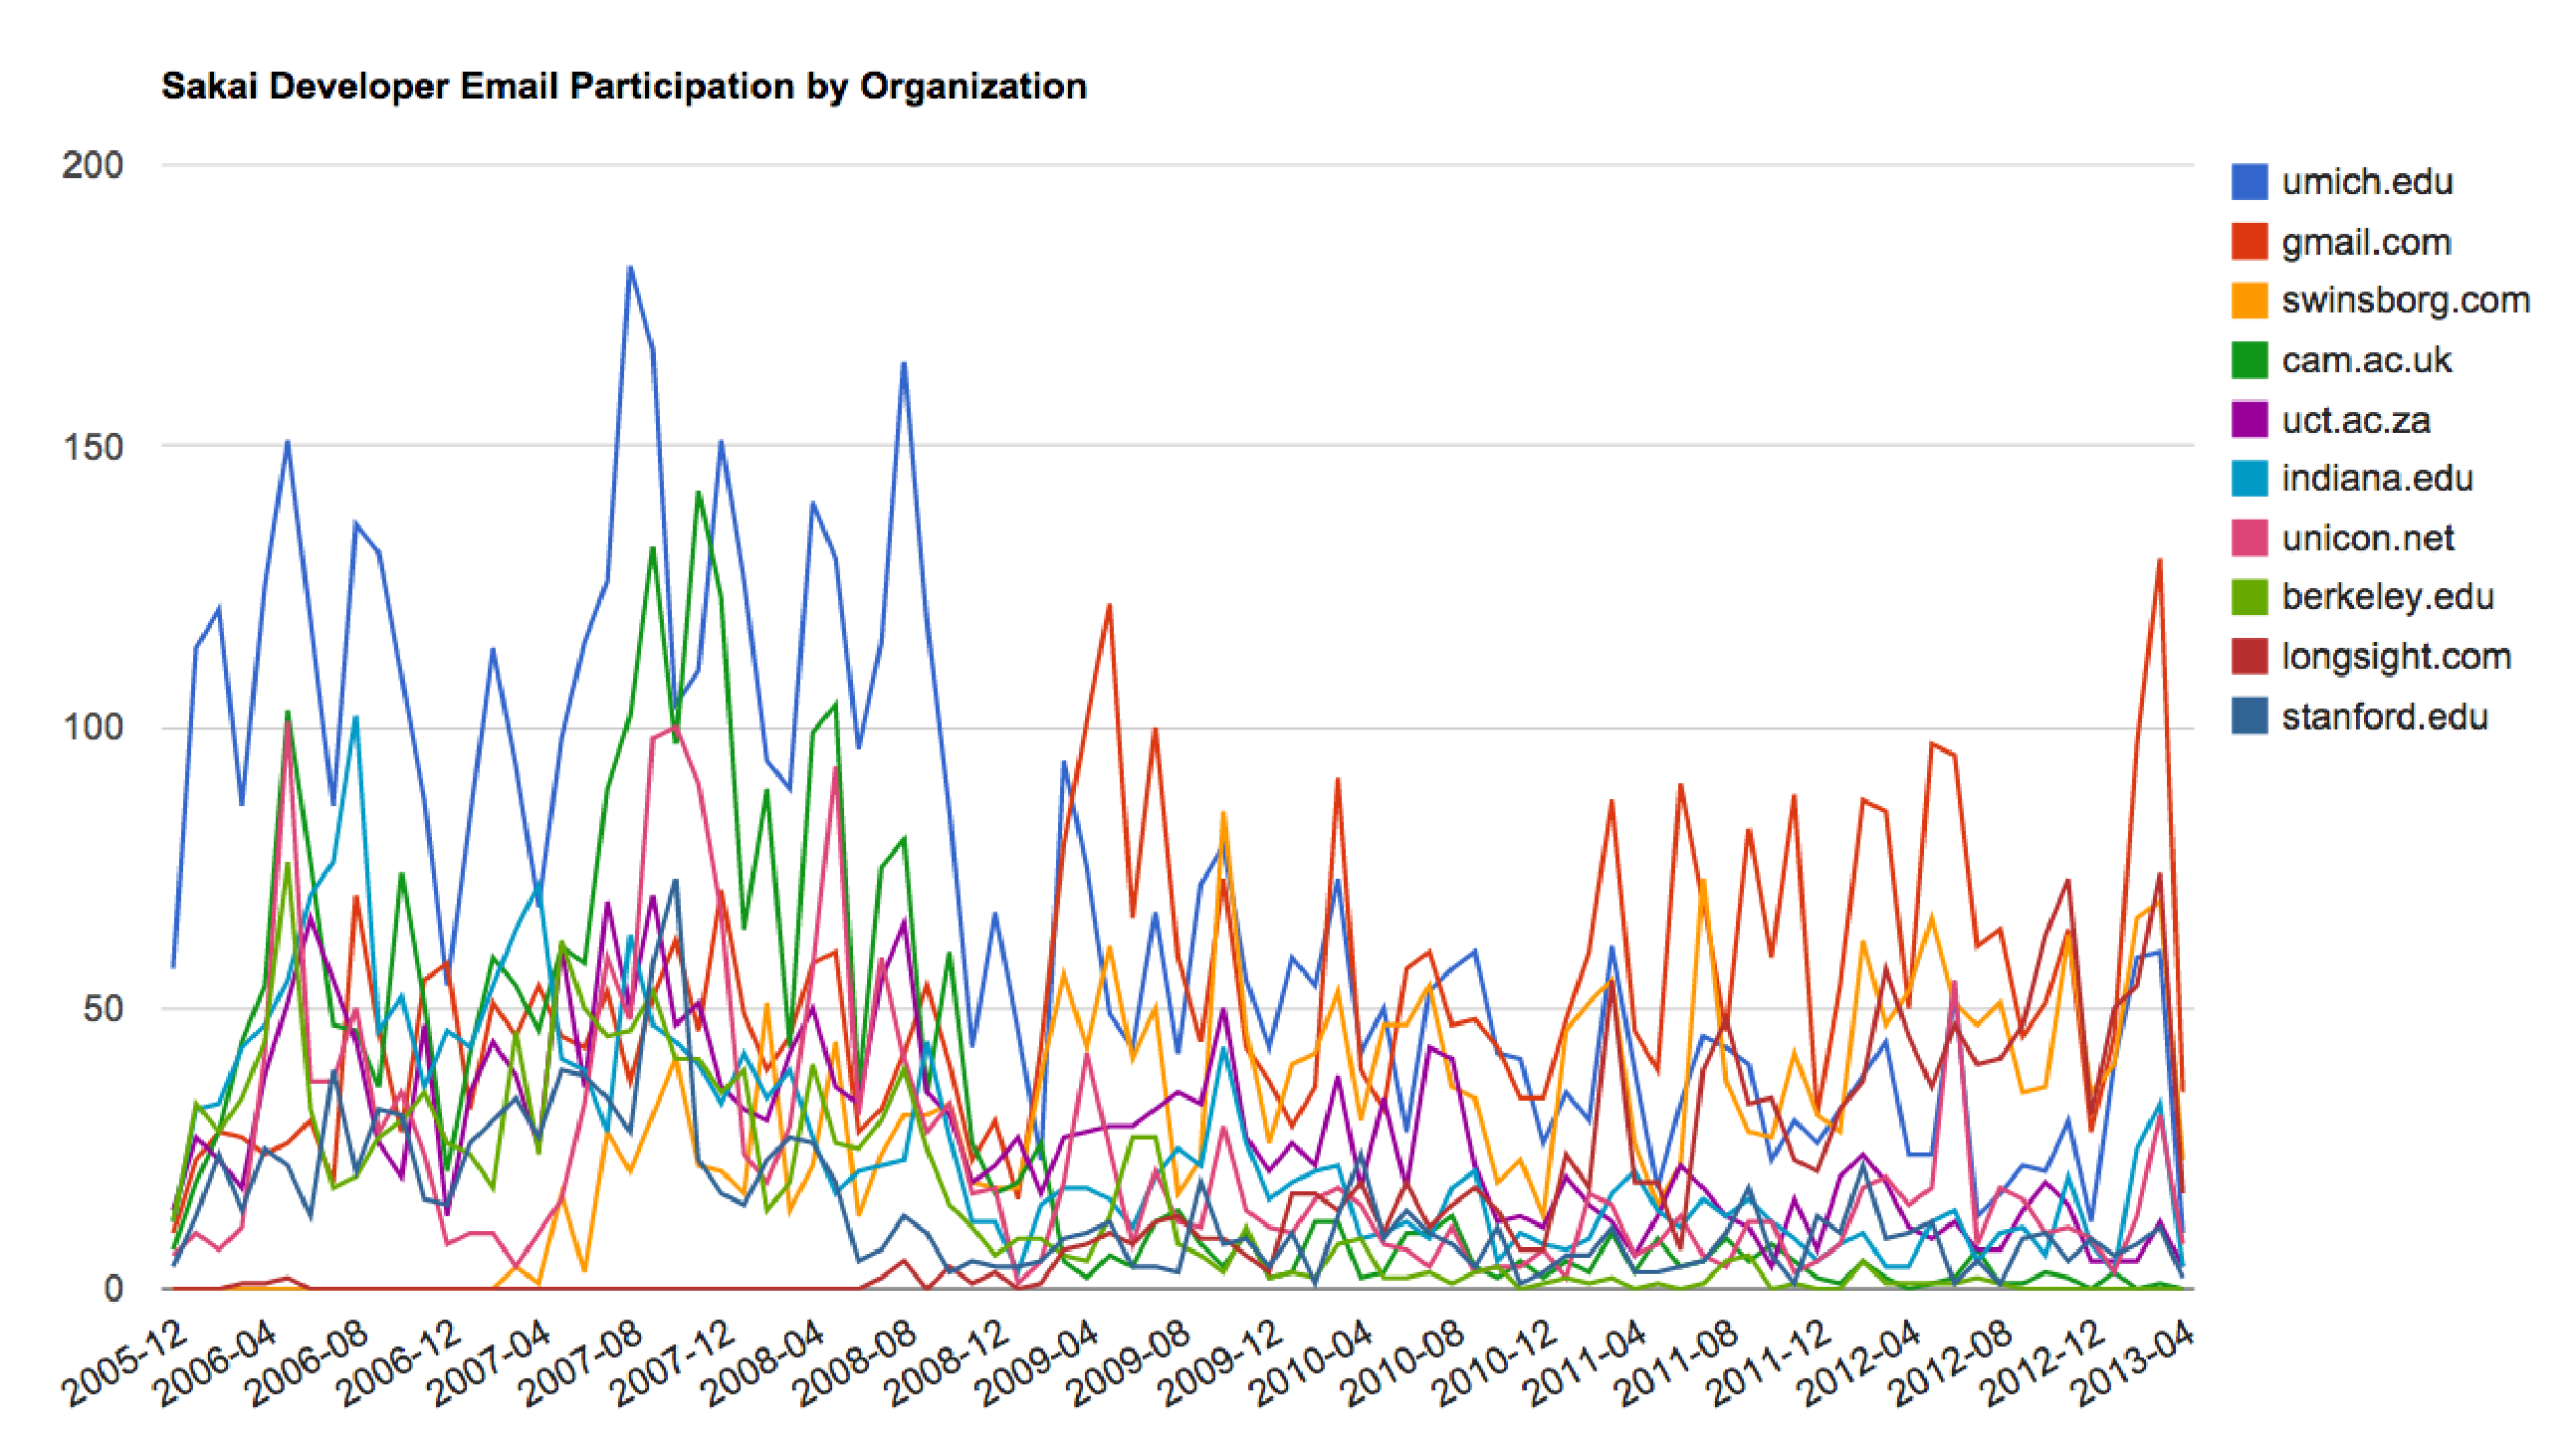
\includegraphics[height=2.50in]{figs2/mailorg.eps}}
\afterfig

Esta aplicación es relativamente compleja y sofisticada, y
dispone de características para realizar recuperación de datos reales, limpieza y visualización.
